\documentclass[a4paper,landscape,extrafontsizes,30pt]{memoir}
\usepackage[utf8x]{inputenc}
\usepackage[english,hebrew]{babel}
\usepackage{graphicx}
\usepackage{verbatim}
\usepackage{url}
\usepackage{bm}
\usepackage{eqnarray}

\textheight=17cm
\textwidth=23cm
\topmargin=-20pt
\headheight=0pt
\oddsidemargin=20pt
\headsep=0pt
\parindent=0pt
\renewcommand{\baselinestretch}{1.1}
\setlength{\parskip}{0.4\baselineskip plus 1pt minus 1pt}

\renewcommand{\familydefault}{\sfdefault}
\pagestyle{empty}


\usepackage[pdflatex]{xcolor}
\pagecolor{green!15!white}

\newcommand*{\slidehead}[1]{\begin{center}\selectlanguage{english}\fcolorbox{black}{green}{\textbf{\rule[-15pt]{0pt}{50pt}\ \ \R{\large #1}\ \ }}\end{center}}

\begin{document}

\selectlanguage{hebrew}

\slidehead{{\Large התחפושות הרבות של אינדוקציה}}


\begin{center}
\textbf{מוטי בן-ארי}


\textbf{המחלקה להוראת המדעים}

\textbf{מכון ויצמן למדע}

\bigskip

{\small\url{http://www.weizmann.ac.il/sci-tea/benari/}}

\vfill

{\scriptsize
\L{\copyright{}\  2019}
מוטי בן-ארי,
לפי
\L{CC BY-SA 3.0}
ייחוס-שיתוף זהה.
}
\selectlanguage{english}
\raisebox{-6pt}{
\includegraphics[width=.12\textwidth]{../by-sa.png}}
\end{center}



\newpage

\slidehead{רקע}

\begin{itemize}
\item
החזרת אינדוקציה לתכנית הלימודים

\item
קורס "המתמטיקה של התכנות" למורים למתמטיקה בתכנית רוטשילד-ויצמן:
\begin{itemize}
\item
המרת בעיות לנוסחאות בלוגיקה ופתרונן על ידי בדיקה ממוחשבת של נכונות הנוסחאות. 
\item
ייצוג טענות נכונות של תכניות על ידי נוסחאות בלוגיקה והוכחת נכונות הטענות.
\end{itemize}
\end{itemize}

\newpage

\slidehead{אינדוקציה מיבנית על נוסחאות בלוגיקה}

\textbf{%
משפט: התכונה
$X$
מתקיימת עבור כל נוסחה.}

\begin{itemize}
\item
טענת בסיס:
$X$
מתקיימת עבור כל נוסחה אטומית
$p$.

\item
הנחת האינדוקציה: 
$X$
מתקיימת עבור 
$A,B$.

\item
הצעד האינדוקטיבי: 
$X$ 
מתקיימת עבור\\
$A\wedge B, A\vee B, A\rightarrow B$.

\item
לפי עיקרון האינדוקציה, 
$X$
מתקיימת לכל נוסחה.

\end{itemize}
\newpage

\slidehead{אינדוקציה מיבנית על סדרת חישוב}

\textbf{%
משפט: התכונה
$X$
מתקיימת בכל מצב במהלך ביצוע של תכנית.}

\vspace{-2ex}

\begin{itemize}
\item
טענת בסיס: 
$X$
מתקיימת במצב התחילי של התכנית.

\item
הנחת האינדוקציה: 
$X$
מתקיימת במצב
$s$.

\item
הצעד האינדוקטיבי:
$X$
מתקיימת בכל מצב 
$s'$
אליו מגיע התכנית מביצוע פקודה במצב
$s$.

\item
לפי עיקרון האינדוקציה, 
$X$
מתקיימת בכל מצב במהלך ביצוע התכנית.
\end{itemize}
\newpage

\enlargethispage{3\baselineskip}

\slidehead{אינדוקציה נמצאת בכל מקום}


\vspace{-4ex}

\begin{center}
\selectlanguage{english}
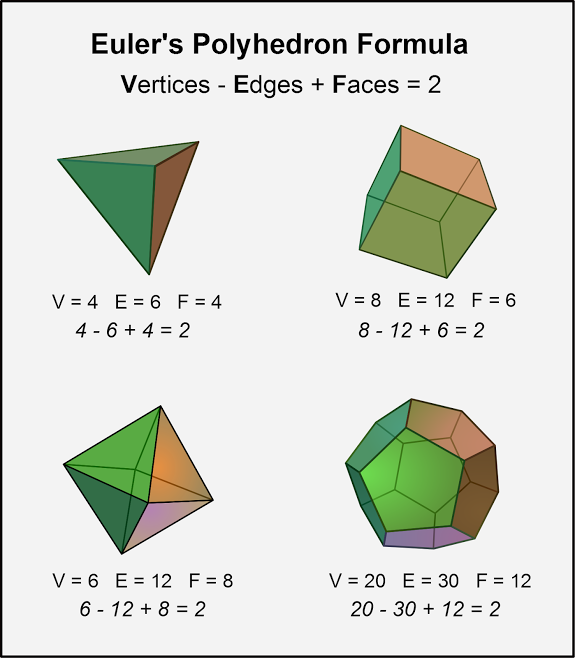
\includegraphics[width=.6\textwidth]{eulers-polyhedron-formula}
\selectlanguage{hebrew}
\end{center}

\newpage

\slidehead{אינדוקציה נמצאת בכל מקום}

\begin{itemize}
\item
טריגונומטריה:
\[
\cos\theta \cdot \cos 2\theta \cdot \cos 4\theta \cdot \cdots \cdot \cos 2^{n-1}\theta = \frac{\sin 2^n\theta}{2^n \sin \theta}\,.
\]
\vspace{-4ex}
\item
לוגיקה: ניתן להמיר כל נוסחה בתחשיב הפסוקים לנוסחה במבנה
\L{3CNF}.
\item
מדעי המחשב: נתון ביטוי רגולרי, ניתן לבנות אוטומט סופי שמקבל את השפה של הביטוי.
\end{itemize}

\newpage

\enlargethispage{3\baselineskip}

\slidehead{קצת נסחפתי}
\vspace{-4ex}
\begin{center}
\selectlanguage{english}
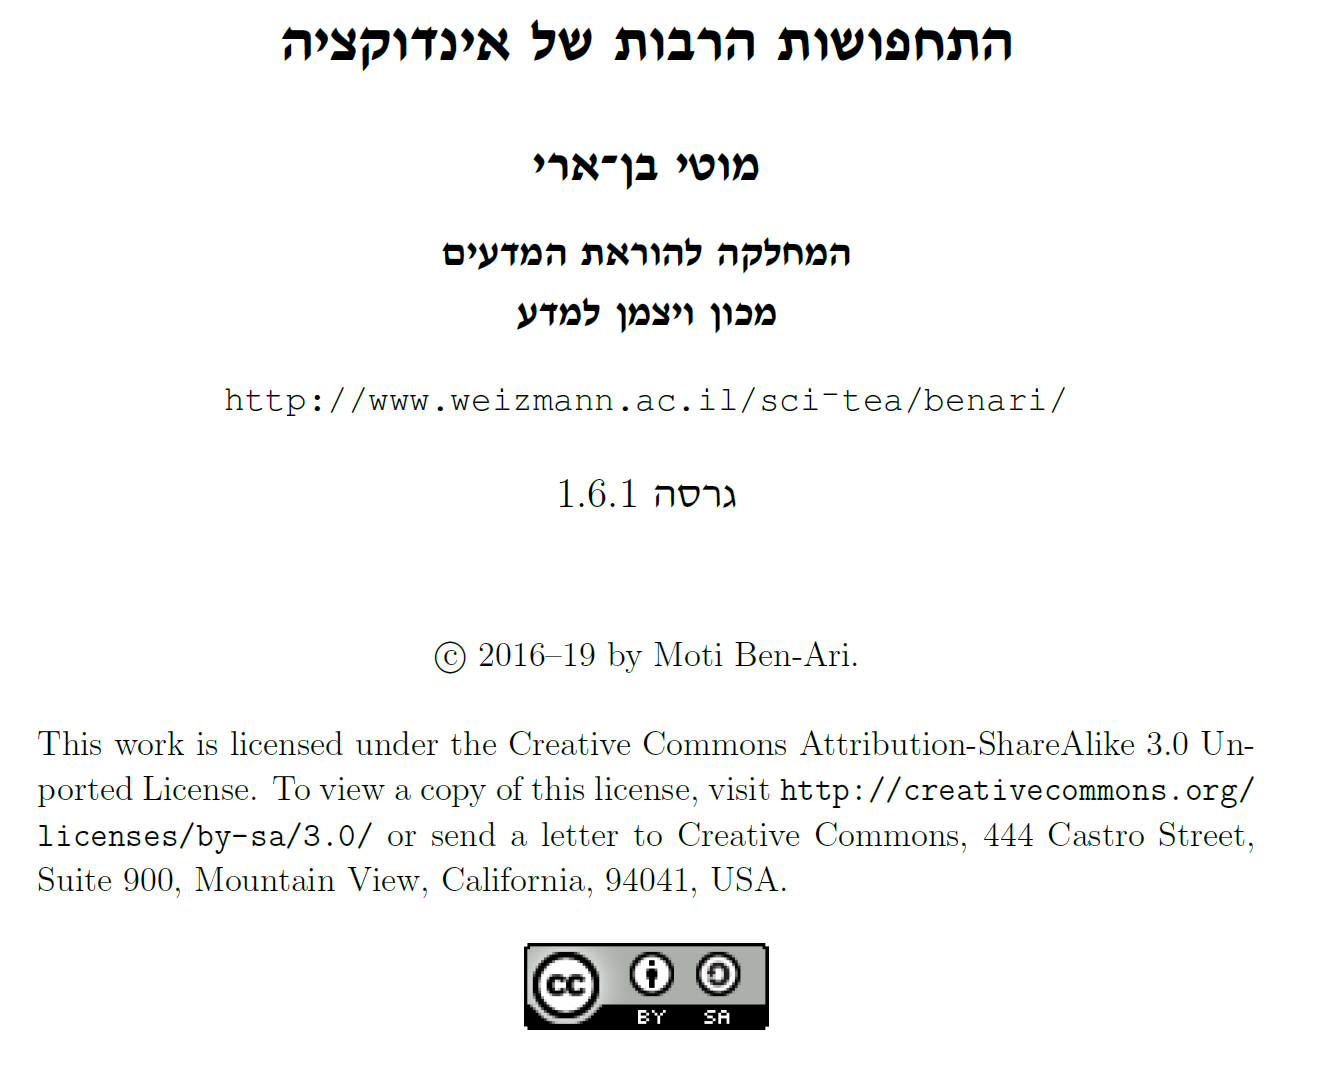
\includegraphics[width=.85\textwidth]{induction}
\selectlanguage{hebrew}
\end{center}

\newpage

\enlargethispage{3\baselineskip}

\slidehead{מישהו נסחף יותר ממני!}
\vspace{-4.5ex}
\begin{center}
\selectlanguage{english}
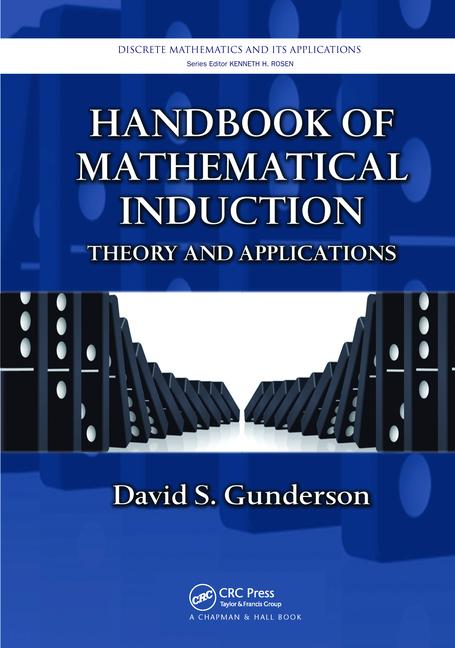
\includegraphics[width=.5\textwidth]{gunderson}
\selectlanguage{hebrew}
\end{center}

\newpage

\slidehead{אי-אפשר בלי אינדוקציה!}

\begin{center}
\L{Fundamental Theorem of Arithmetic}
\end{center}

\bigskip

\textbf{%
משפט: ניתן לפרק כל מספר שלם למכפלה של\\מספרים ראשוניים בדרך אחת )הסדר לא חשוב(.}
\[
337,500 = 2^2 \cdot 3^3 \cdot 5^5\,.
\]

\newpage


\slidehead{אי-אפשר בלי אינדוקציה!}

\vspace{-2ex}
\begin{center}
\textbf{הוכחת הקיום של פירוק למספרים ראשוניים}
\end{center}
\vspace{-4ex}

\begin{itemize}
\item
טענת בסיס: אם n ראשוני, אין מה להוכיח.
\vspace{-1ex}
\item
הנחת האינדוקציה: כל
$k\leq n$
ניתן לפרק למכפלה של מספרים ראשוניים.
\vspace{-1ex}
\item
הצעד האינדוקטיבי: אם
$n+1$
ראשוני, המשפט נכון. אחרת,
$n+1=n'\cdot n''$
כאשר
$n',n'' \leq n$.
לפי הנחת האינדוקציה )אינדוקציה שלמה( יש ל-%
$n+1$
פירוק למכפלה של מספרים ראשוניים.
\vspace{-1ex}
\item
לפי עיקרון האינדוקציה, המשפט נכון )אינדוקציה 1(.

\end{itemize}
\newpage

\slidehead{אי-אפשר בלי אינדוקציה!}

\begin{center}
\textbf{הוכחת פירוק בדרך אחת}
\end{center}
\textbf{%
הזהות של
\L{B\'{e}zout}}:
\setlength{\extrarowheight}{6pt}
\begin{equationarray*}{rcl}
\gcd(n_1,n_2) &=& a\cdot n_1+b\cdot n_2\\\\
\gcd(15,81) &=& 	11\cdot 15 + (-2)\cdot 81 = 165 - 162= 3\\
\gcd(25,81) &=& 13\cdot 25 + (-4) \cdot 81 = 325-324=1\,.
\end{equationarray*}
 הוכחה באמצעות עיקרון הסדר הטוב )גם אינדוקציה 2(.
\newpage

\slidehead{אי-אפשר בלי אינדוקציה!}

\textbf{%
הלמה של אוקלידס:
אם
$p$
ראשוני מחלק את\\
$n=n_1\cdot n_2$,
אזי 
$p$
מחלק את
$n_1$
או
$p$
מחלק את
$n_2$.}

\bigskip
הוכחה באמצעות הזהות של 
\L{B\'{e}zout}.

\newpage

\slidehead{אי-אפשר בלי אינדוקציה!}
\textbf{%
הלמה הכללית של אוקלידס: אם
$p$
ראשוני מחלק את
$n=n_1\cdot n_2\cdots n_k$,
אזי 
$p$
מחלק אחד מ-%
$1\leq i \leq k,\;n_i$.}

הוכחה: 
$k=2$
הוא הלמה של אוקלידס.

$k>2$:
\vspace{-2ex}
\[
n=(n_1\cdot n_2\cdots n_{k-1})\cdot n_k\,.
\]
לפי הלמה של אוקלידס,
$p$
מחלק את
$n_k$
או
$p$
מחלק את
$n_1\cdot n_2\cdots n_{k-1}$.
לפי אינדוקציה שלמה,
$p$
מחלק את אחד מ-%
$1\leq i \leq k-1,\;n_i$
)אינדוקציה 3(.

\newpage
\slidehead{אי-אפשר בלי אינדוקציה!}

נניח בשלילה שעבור 
$\{p_i\}\neq\{q_j\}$
ראשוניים:
\[
n=p_1\cdots p_k = q_1\cdots q_m\,.
\]

\vspace{-4ex}

לפי הלמה הכללית של אוקלידס,
$p_1$
מחלק את
$q_i$
עובר
$1\leq i\leq m$.
\textbf{ללא הגבלת הכלליות}
$p_1$
מחלק את
$q_1$.

$p_1,q_1$
ראשוניים, ולכן
$p_1=q_1$
וניתן לצמצם את המכפלה.

\textbf{נמשיך באותה דרך}
עד שייגמרו כל ה-
$p_i$
או כל ה-%
$q_j$.

\newpage

\slidehead{אינדוקציה סמויה}

\begin{itemize}
\item
הביטוי
\textbf{ללא הגבלת הכלליות}
מסתיר אינדוקציה )4( תוך שימוש בחוקי החילוף והקיבוץ:
\vspace{-1ex}
\[
n= (q_1\cdot q_2) \cdot (q_3) \cdot (q_4\cdot q_5 \cdot q_6) \cdots\,.
\]
\vspace{-4ex}
\item
הביטוי
\textbf{נמשיך באותה דרך}
מסתיר אינדוקציה )5(.

\end{itemize}

קיימת הוכחה אינדוקטיבית של 
\L{Zermelo}
ללא שימוש בזהות של
\L{B\'{e}zout}.

\newpage

\slidehead{עיקרון הסדר הטוב}

\textbf{%
עיקרון הסדר הטוב: בכל קבוצה של מספרים שלמים חיוביים קיים איבר קטן ביותר.}

\textbf{%
משפט: אם עיקרון הסדר הטוב נכון, גם עיקרון\\האינדוקציה נכון.}

\textbf{%
הוכחה:}
נניח בשלילה שאינדוקציה לא נכונה. תהי
$S$
קבוצת המספרים עבורם אינדוקציה לא נכונה, כלומר:
$X(1)$
נכונה, אם מניחים ש-%
$X(n)$
נכונה, אזי
$X(n+1)$
נכונה, אבל עבור כל
$k_i\in S$,
$X(k_i)$
לא נכונה.

\newpage

\slidehead{עיקרון הסדר הטוב}

\[
\selectlanguage{english}
\begin{array}{cccccccc}
%\begin{array}{llllllll}
X(1) & X(2) & X(3)& X(4) &\cdots& X(56) &X(57) &\cdots\\
\surd&\surd&\surd&\surd&\surd&\surd&\times&\surd\\
\\
X(127)&\cdots &X(158) &X(159) &\cdots &X(542)&\cdots\\
\surd&\surd&\times&\times&\surd&\times&\surd\\
\end{array}
\selectlanguage{hebrew}
\]
$S=\{158,57,542,159,\cdots\}$.
לפי עיקרון הסדר הטוב, קיים איבר הקטן ביותר בקבוצה, כאן
$57$,
ולכן 
$X(56)$
נכונה. לפי הצעד האינדוקטיבי
$X(57)$
נכונה. סתירה!

\newpage


\slidehead{עיקרון הסדר הטוב}
\enlargethispage{\baselineskip}

\textbf{%
משפט: אם עיקרון האינדוקציה נכון, עיקרון הסדר הטוב נכון.}

הוכחה: תהי
$S$
קבוצה
\textbf{לא-ריקה}
של המספרים החיוביים. נניח שאין איבר קטן ביותר בקבוצה 
$S$.
\[
S = \{\ldots,37,175,539,\ldots\}\,.
\]
נגדיר:
%$X(n)$:
%\begin{center}
$X(n)$
נכונה אם לכל 
$k\leq n$, $k$
\textbf{אינו}
איבר של
$S$.
%\end{center}

\newpage

\slidehead{עיקרון הסדר הטוב}

\vspace{-2ex}
\[
\selectlanguage{english}
\begin{array}{c@{\hspace{1em}}c@{\hspace{1em}}c@{\hspace{1em}}c@{\hspace{1em}}c@{\hspace{1em}}c}
X(1) & X(2) & X(3) & \cdots &X(n)&X(n+1)\\
1\not\in S&2\not\in S&3\not\in S&&n\not\in S&(n+1)\: \bm{?\!\in?} \:S\\
\end{array}
\selectlanguage{hebrew}
\]
\vspace{-3ex}

\begin{itemize}
\item
טענת בסיס: 
$1$
הוא המספר החיובי הקטן ביותר, ולכן אם אין מספר קטן ביותר ב-%
$S$,
$1$
לא יכול להיות ב-%
$S$,
ו-%
$X(1)$
נכונה.
\end{itemize}

\newpage

\slidehead{עיקרון הסדר הטוב}

\vspace{-2ex}
\[
\selectlanguage{english}
\begin{array}{c@{\hspace{1em}}c@{\hspace{1em}}c@{\hspace{1em}}c@{\hspace{1em}}c@{\hspace{1em}}c}
X(1) & X(2) & X(3) & \cdots &X(n)&X(n+1)\\
1\not\in S&2\not\in S&3\not\in S&&n\not\in S&(n+1)\: \bm{?\!\in?} \:S\\
\end{array}
\selectlanguage{hebrew}
\]
\vspace{-4ex}

\begin{itemize}
\item
הנחת האינדוקציה:
$X(k)$
נכונה, לכן 
$k\leq n$.

\item
הצעד האינדוקטיבי: לפי הנחת האינדוקציה, אם

$n+1$
ב-%
$S$,
אזי 
$n+1$ 
הוא האיבר הקטן ביותר ב-%
$S$.
סתירה. לכן,
$n+1$
אינו ב-%
$S$
ו-%
$X(n+1)$
נכונה.
\item
לפי אינדוקציה,
$X(n)$
נכונה לכל המספרים החיוביים, כלומר,
$S$
היא קבוצה
\textbf{ריקה}.
סתירה.
\end{itemize}

\newpage

\slidehead{פנינה}
\textbf{משפט: כל מספר פיבונצ'י רביעי מתחלק בשלוש!}
\[
\begin{array}{l}
f_1 =1,\; f_2 = 1,\; f_n = f_{n-1} + f_{n-2}\,.\\
\\
1, 1, 2, \bm{3}, 5, 8, 13, \bm{21}, 34, 55, 89, \bm{144},233,377,610,\ldots\,.
\end{array}
\]
הוכחה:

טענת בסיס:
$f_4=3$.

הנחת האינדוקציה: 
$f_{4n}$
מתחלק ב-%
$3$.
\newpage

\slidehead{פנינה}

\vspace{-1ex}
הצעד האינדוקטיבי:
\vspace{-2ex}
\begin{eqnarray*}
f_{4(n+1)} &=& f_{4n+4}\\
&=& f_{4n+3}+f_{4n+2}\\
&=& (f_{4n+2}+f_{4n+1})+f_{4n+2}\\
&=& ((f_{4n+1}+f_{4n})+f_{4n+1})+f_{4n+2}\\
&=& ((f_{4n+1}+f_{4n})+f_{4n+1})+(f_{4n+1}+f_{4n})\\
&=& 3f_{4n+1}+2f_{4n}\,.
\end{eqnarray*}
$3f_{4n+1}$
מתחלק ב-%
$3$
ולפי הנחת האינדוקציה גם
$f_{4n}$.


תרגיל: 
$f_n<\left(\frac{7}{4}\right)^n$.


\newpage

\slidehead{מסקנות}

\begin{itemize}
\item
אינדוקציה היא לא תבנית קבועה אלא מושג בסיסי במתמטיקה.
\item 
רצוי שמורים יכירו אינדוקציה לעומקה ולרוחבה.
\item
הוראת עיקרון הסדר הטוב עשויה להקל על התלמידים במפגשם הראשון עם אינדוקציה.


\end{itemize}
\end{document}